\documentclass[11pt,letterpaper]{article}
\usepackage[T1]{fontenc}
\usepackage{lmodern}
\usepackage[margin=0.94in,top=0.86in,bottom=0.91in,headheight=14pt]{geometry}
\usepackage{amsmath,amssymb,amsthm,mathtools,graphicx,booktabs,array,microtype,xcolor,fancyhdr}
\usepackage[hyphens]{url}
\definecolor{ink}{HTML}{173A48}
\definecolor{blueink}{HTML}{145C73}
\usepackage[colorlinks=true,linkcolor=ink,citecolor=ink,urlcolor=blueink,pdfauthor={OpenAI},pdftitle={Finite observations of continuous mathematics in iPRA}]{hyperref}
\newtheorem{theorem}{Theorem}[section]
\newtheorem{lemma}[theorem]{Lemma}
\newtheorem{proposition}[theorem]{Proposition}
\newtheorem{corollary}[theorem]{Corollary}
\theoremstyle{definition}\newtheorem{definition}[theorem]{Definition}
\newcommand{\ipra}{\ensuremath{\mathsf{iPRA}}}
\newcommand{\N}{\mathbb N}
\newcommand{\Q}{\mathbb Q}
\newcommand{\R}{\mathbb R}
\newcommand{\norm}[1]{\left\lVert#1\right\rVert}
\newcommand{\eps}{\varepsilon}
\setlength{\parindent}{1.2em}
\setlength{\parskip}{2pt}
\setcounter{tocdepth}{1}
\pagestyle{fancy}\fancyhf{}
\fancyhead[L]{\small\color{ink}Finite observations of continuous mathematics}
\fancyhead[R]{\small\color{ink}\ipra}
\fancyfoot[C]{\small\thepage}
\renewcommand{\headrulewidth}{0.3pt}
\emergencystretch=2em
\begin{document}
\thispagestyle{plain}
{\small\bfseries\color{blueink} CONSTRUCTIVE MATHEMATICS \hfill NOVEMBER 2026}\par
\vspace{14pt}
{\fontsize{26}{30}\selectfont\bfseries\color{ink}Finite observations of continuous\\[2pt] mathematics in iPRA\par}
\vspace{7pt}
{\large Metric kernels, continuous quantifiers, exact crossings, and residues\par}
\vspace{13pt}
\noindent A finite calculation can determine an infimum to high accuracy while its minimizing arguments move between distant points. This distinction governs which parts of a continuous proof can be carried out in intuitionistic primitive recursive arithmetic. We give a comparison principle for finite observations, a condition for extracting a point from local witnesses, and four applications. For metric kernels we compute composition and test equality by distance probes. For continuous logic an atomic error bound survives every quantifier in a fixed nonexpansive formula. For paths crossing a Jordan curve we give a condition producing actual parameter names and verify it for polynomial paths under an algebraic hypothesis. For residues we move rational contours around separated singularities given by regular names. Each use of a continuous object is traced to rational operations, finite bounds, or explicit hypotheses about a presentation.\par
\vspace{7pt}
\noindent The Lean files include derivations in ProveIt's object calculus and ordinary Lean theorems about the finite algorithms. Section~\ref{sec:verification} states the scope of each check.
\vspace{7pt}
\tableofcontents
\medskip
\noindent\small\textbf{Three values computed in the text.}
An interval-data set first admits a global short fit at error \(1/3\). Three centers cover the unit interval at optimal radius \(1/6\). A rectangular contour separating the two roots of \(z^2-2\) has integral \(\pi i/\sqrt{2}\) for the reciprocal polynomial.\normalsize
\clearpage
\section{What a continuous assertion means in arithmetic}
\label{sec:framework}

Take the repository's ordinary \ipra{} with intuitionistic first-order logic with equality, a symbol with defining equations for every primitive-recursive (PR) definition, the successor axioms, and quantifier-free induction. Its Lean judgement is \( \Gamma\vdash_{\mathsf{PRAAx}}\phi \). Our snapshot is \texttt{5f3be02388} of ProveIt. The \href{https://github.com/VladimirReshetnikov/ProveIt/blob/5f3be02388442f16487d2dc5c2529961dd783d2b/Logic/PrimitiveRecursiveArithmetic/Derivations/FINITE-DEMAND-CLAIMS.md}{finite-demand audit} already records object derivations for bounded reflection, changing-parameter recursion, and several finite Hausdorff estimates. In particular, its aggregate optimization works with approximate support witnesses. The \href{https://github.com/VladimirReshetnikov/ProveIt/tree/5f3be02388442f16487d2dc5c2529961dd783d2b/Logic/PrimitiveRecursiveArithmetic/docs/proofs/foundations/ipra_categorical_methods}{categorical packet} treats finite Kan extensions, gluing and the difficulty of choosing a coherent branch. We use these as starting points. A metric kernel below has a continuum of possible intermediate points, and its finite composites need only agree up to a computable error.

\paragraph{The interpretation.}
A presentation has a decidable PR domain of dense codes \(D\subseteq\N\), total PR operations (with defaults on invalid codes) and arithmetical proofs of their laws on valid inputs. Different spaces can have different domains. A rational pseudometric on \(D\) gives a convenient common case. For an external, fixed PR program \(x(p,i)\), with numerical parameter \(p\), the assertion that it names a point reads
\[
 \operatorname{Reg}(x,p)\quad\Longleftrightarrow\quad
 \forall i,j\quad x(p,i)\in D\ \land\
 d(x(p,i),x(p,j))\le 2^{-i}+2^{-j}.
\]
The omitted membership for \(j\) follows by instantiation. In this formula \(x\) is the function symbol for the given program. A complete metric space may serve as the external interpretation. The formulas themselves need only dense codes. For two regular names \(x,y\), equality means
\(\forall k\,\exists N\,\forall i,j\ge N,\ d(x_i,y_j)\le 2^{-k}\).
Equivalently \(d(x_i,y_j)\le 2^{-i}+2^{-j}\) for all \(i,j\). For the forward direction insert sufficiently fine \(x_t,y_u\) between \(x_i,y_j\), then use the decidable order of the rational endpoints. If the displayed bound failed, choose the errors \(2^{-t},2^{-u}\) and the cross-distance smaller than one quarter of the positive rational gap. The reverse implication takes \(N=k+1\). Thus equivalence of regular names has a universal formulation with a decidable matrix.

An operation on names is a proof-generating construction on fixed input programs. Its conclusions assert regularity and independence of equivalent representations. A claim about every represented input is a schema of these arithmetical conclusions. A single uniform family is possible when the presentations are already given by one fixed PR program with data parameters. An arbitrary code for a PR program is insufficient. A PR universal evaluator \(U(e,x)\) total and correct on every unary PR code would make \(x\mapsto U(x,x)+1\) PR, contradicting its own entry. We pass finite tables as data when a signature or index set is truly variable.

\paragraph{Coding and comparison.}
Use the repository's pairing and finite-sequence definitions. An alternative concrete coding stores zero for nil and \(1+\langle a,s\rangle\) for cons, with Cantor pairing. Projections are bounded searches through the code, and taking at most code-many tails terminates for every code. Integers are differences of two naturals. Rational numbers are a signed numerator and a positive denominator. Products of denominators convert finitely many rational comparisons into integer ones, including strict inequalities. The matrices below are finite lists of rows. A precision, an index, a numerator or a length in such a matrix can be an object variable. All malformed inputs have a fixed output supplied by the program. Each assertion about the intended semantics retains its input guards.

\subsection{A principle for transferring an estimate}
\label{sec:principle}
At stage \(i\), an experiment has a finite nonempty list of legal answers. Pair two experiments by a decidable relation \(R\) between their answers. In both directions, every legal answer must have a relative. For a rational terminal observable \(F\) the useful condition is a bound
\[
 |F_i(u)-F_j(v)|\le b\qquad(uRv).
\]
The relation can depend on the previous answers and the stage pair. One only needs the two coverage implications at the histories being compared. For a fixed finite expression built from these observations, form its value as follows. At a choice node take the minimum or maximum of its continuations, and at a deterministic node apply a rational connective \(C\). Suppose a PR function \(\omega_C(e_1,\ldots,e_s)\) bounds the output discrepancy when the inputs differ by at most \(e_1,\ldots,e_s\), with the same domain guard on both evaluations.

\begin{theorem}[Comparison of two finite evaluations]\label{thm:compare}
Assign a bound to each pair of related terminal histories. At a choice node take any common upper bound for the bounds on related child pairs. At a deterministic node apply \(\omega_C\). The resulting bound at the root bounds the discrepancy of the two evaluations. In particular, if all terminal discrepancies are at most \(b\) and all connectives are nonexpansive in the maximum metric, the root discrepancy is at most \(b\), independently of nesting.
\end{theorem}
\begin{proof}
At a minimum node select the least index attaining the second minimum. Coverage supplies a matching first answer. The first minimum is at most the value at that answer, which is at most the second minimum plus the child bound. Exchange the experiments for the other inequality. A maximum uses the maximizing answer in the first experiment to bound the first maximum from above, and then exchanges experiments. A deterministic node uses its stated inequality. These steps prove the claim by induction on the external expression. Each terminal comparison is used only at related histories. Locally one cover gives one inequality, with the direction reversed at maxima. To propagate a single inequality through a whole tree, use the required direction at each binder and a suitable monotonicity law at each deterministic node. An empty choice has no selected index, which explains the nonemptiness condition.
\end{proof}

If all stage-pair bounds are \(b_{ij}\le c(2^{-i}+2^{-j})\), taking \(i=k+s\) with \(2^s\ge c\) constructs a regular name for the result. When a terminal conclusion is a discrete label, a separate separation inequality can identify it exactly. For example, two integer certificates within a proven distance \(<1\) are equal. Precision loss can also be incurred in changing coordinates. The contour argument in Section~\ref{sec:namedresidue} uses clearance for precisely this purpose.

\paragraph{A value versus a point.}
A different invariant turns local witnesses into a point. Start with a validated state and suppose a fixed PR program sends each validated state \(s_i\) to \(s_{i+1}\) and supplies a dense code \(p_i\). Assume a PR rational bound \(b_i\ge0\), a PR rate \(g(k)\) with \(b_{g(k)}\le2^{-k}\), and verified finite implications giving \(d(p_i,p_j)\le b_i\) whenever \(j\ge i\). Then \(k\mapsto p_{g(k)}\) is regular. Compare the two selected indices in order, and use the small bound at the earlier one. If a residual \(F\) has a supplied modulus of uniform continuity and the selected \(F(p_{g(k)})\) tend to zero at a PR rate, its value at the resulting name is zero. Evaluate \(F\) on a sufficiently fine representative so its evaluation error and residual are each below half the requested tolerance. This is the mechanism behind the crossing proof. The Cantor-space example in Section~\ref{sec:continuous-models} explains why a PR answer at each stage alone cannot replace it.

\paragraph{Changing a coordinate chart by a name.}
A geometric construction may require rational grid vertices even when its natural origin is a represented point. Write \(h_n=2^{-n}\). For a query \(t\) in the new chart, let \(q_m(t)\) be PR rational coordinates in the original chart, regular in \(m\). Suppose that for \(m\ge B(t)\) these coordinates lie in a carrier where the same evaluator and modulus are certified. Assume \(B\) is PR and the old rational evaluator satisfies
\[
 d(u,v)\le 2^{-\mu(l)}
 \ \Longrightarrow\quad
 |F_i(u)-F_j(v)|\le 2^{-l}+h_i+h_j.
\]
The norm may also be a coded vector norm satisfying the triangle inequality. Define
\[
 a(k,t)=\max\{B(t),1+\mu(k+2)\},\qquad
 G_k(t)=F_{k+2}\big(q_{a(k,t)}(t)\big).
\]
For \(T\ge a(k,t)\), regularity puts \(q_T(t)\) within \(2h_{a(k,t)}\) of the sampled coordinate. Consequently \(|G_k(t)-F_b(q_T(t))|\le 2h_{k+2}+h_b\) for every \(b\). Insert the same \(T,b\) between two evaluations at precisions \(k,j\), then discard the arbitrarily small \(2h_b\) by rational comparison. This proves regularity of \(G\). To transport an identity among finitely many queries, use \(T\) at least the maximum of their demands and evaluate the original identity there. For example, an equality of two weighted sums with rational weights \(w_\nu\) incurs at most \(\sum_\nu |w_\nu|(2h_{k+2}+h_b)\), taking the sum over terms on both sides. A positive target error fixes both precisions by bounded search using its rational denominator and the sum of weights. Products use \(|ab-a'b'|\le |a|\,|b-b'|+|b'|\,|a-a'|\) with supplied magnitude bounds. Strict guards require a positive margin before moving the coordinates. In Section~\ref{sec:namedresidue} the carrier is a shell, the chart change preserves differences exactly at a common \(T\), and an incidence identity identifies the two contour boundaries. The same rule applies to charted observables on real intervals or presented manifolds wherever the carrier and bounds are supplied.

\paragraph{Induction budget.}
For a fixed expression the tree induction is in the metatheory. It constructs a finite proof for that expression. The object inductions in a bounded scan use a Boolean prefix invariant, such as the assertion that the winner lies in the prefix and its value is no larger than every entry seen. A bounded universal is a fold of Boolean conjunction, with prefix recursion on the length. Reflect the bounded comparison to its bit using the fixed-formula bounded-reflection theorem, use the fold equations for base and step, then apply quantifier-free induction to equality of the bit with one. A coverage premise is consulted at the particular entry under discussion by existential elimination. For an iterated state use a componentwise validity bit and, when bounds involve earlier rows, a bounded scan through the computed prefix. Universal numerical parameters outside these loops are generalized after the induction. Claims about input programs involving unbounded quantifiers remain explicit hypotheses.

\section{Composition and reconstruction of metric kernels}\label{sec:category}

Consider a traveler going from \(x\) to \(z\) through a point \(y\) of a compact metric space. The optimal cost is an infimum over \(y\). One can compute it and compose further such trips even if no program selects optimal intermediate points. This gives an effective category of the metric distributors underlying \href{https://www.tac.mta.ca/tac/reprints/articles/1/tr1abs.html}{Lawvere's enriched metric spaces}. We give error estimates for its composition and recover a distributor from its action on scalar distance observations.

\subsection{The category on presentations}

For each object \(X\) give a nonempty dense rational pseudometric presentation \(D_X\) as in Section~\ref{sec:framework}. At each \(i\) supply a nonempty PR finite list \(N^X_i\subset D_X\) with proved covering radius \(h_i=2^{-i}\) on \(D_X\). This means \(\forall x\in D_X\,\exists b<|N^X_i|,\ d_X(x,N^X_i[b])\le h_i\). A PR selector follows by bounded rational search. Nesting of nets is optional. A morphism \(K:X\to Y\) is a fixed program giving nonnegative rational observations \(K_i(x,y)\), with the arithmetical law
\begin{equation}
 |K_i(x,y)-K_j(x',y')|\le d_X(x,x')+d_Y(y,y')+h_i+h_j .
 \label{eq:cost-law}
\end{equation}
Two morphisms represent the same arrow when their names agree at all pairs of dense codes. At named endpoints the sample at precision \(k\) is \(K_{k+2}(x_{k+2},y_{k+2})\). Its cross-stage bound is at most \(3(h_k+h_j)/4\) by regularity in the two coordinates and the table. Equivalent regular inputs give the same result by \eqref{eq:cost-law}. Each represented kernel is separately 1-Lipschitz. Conversely, an externally given nonnegative such kernel together with a uniform PR sampler of error \(h_i\) and proofs of these estimates gives precisely the required arithmetic data. Rational pseudometrics, circle charts and cubes already give infinite examples. For clarity we use finite costs.

For \(H:Y\to Z\) define a raw table and its shifted representative by
\begin{equation}
 C_i(x,z)=\min_{b\in N^Y_i}\big(K_i(x,b)+H_i(b,z)\big),\qquad
 (H\circ K)_k=C_{k+2}.
 \label{eq:convolution}
\end{equation}
The identity on \(X\) is the exact table \(d_X(x,x')\) at all levels.
\begin{theorem}[Effective composition]\label{thm:cat}
Equation \eqref{eq:convolution} satisfies \eqref{eq:cost-law}, respects equivalence of representatives and gives an associative composition with the stated identities on equivalence classes. Its represented value is the infimum of \(K(x,y)+H(y,z)\) over represented \(y\). The finite minimizer at each precision is an approximate witness.
\end{theorem}
\begin{proof}
Relate the intermediate grids at distance at most \(\max(h_i,h_j)\). They cover each other in both directions. For related \(b,b'\) the two costs differ by at most
\[
 d_X(x,x')+d_Z(z,z')+2\max(h_i,h_j)+2(h_i+h_j).
\]
Theorem~\ref{thm:compare} gives the same bound for \(C_i,C_j\). The last two terms are at most \(4(h_i+h_j)\). Shifting by two gives the defining law including its exact coefficient on the free endpoint distances.

Here and below a symbol without a stage subscript is shorthand for the real determined by its regular observations. In particular \(|K_i(x,y)-K(x,y)|\le h_i\) at dense codes, by comparison with all later stages. Write \(V\) for the name in \eqref{eq:convolution}. For a dense \(y\), a grid point within \(h_i\) gives
\[
 C_i(x,z)\le K(x,y)+H(y,z)+4h_i.
\]
Passing to arbitrary precision gives \(V\le K(x,y)+H(y,z)\). A represented \(y\) follows by substituting its dense approximants and using their regularity. Conversely, let \(b_i\) attain \(C_i\). Then \(K(x,b_i)+H(b_i,z)\le C_i+2h_i\). Every lower bound for all dense candidates is therefore at most \(V\). More quantitatively, since \(V\) is already a lower bound and a greatest lower bound, \(C_i-4h_i\) is a lower bound by the preceding covering inequality, so
\[
 -2h_i\le C_i-V\le 4h_i,\qquad
 K(x,b_i)+H(b_i,z)\le V+6h_i.
\]
This proof constructs the infimum using only comparisons of names. Its lower-bound and approximate-witness properties give uniqueness and invariance under equivalent input kernels.

For an identity on the left or the right the triangle bound for a kernel makes each candidate at least the desired kernel entry. Taking the unchanged endpoint as intermediate gives equality. For associativity consider three arrows \(K,H,J\) with endpoint pair held fixed. The finite flat sum has entries \(K(x,b)+H(b,c)+J(c,w)\). The two nested minima of an exact finite rectangle are equal. Indeed, evaluating either at a minimizing pair of the other proves one inequality in each direction. We give the error argument also, since the two expressions in \eqref{eq:convolution} use different levels. Put \(s=k+2\) and use \(N_s^Y,N_s^Z\) and all three stage-\(s\) tables for the flat calculation. In either parenthesization exactly one intermediate grid and two tables are at level \(s+2\). Replacing them by level \(s\) changes the inner minimum by at most \(2h_s+2(h_s+h_{s+2})\) by the two-grid calculation, uniformly in the unchanged intermediate point. Taking the outer minimum preserves this bound. The difference of parenthesizations is at most twice this number, tending to zero with a PR rate. All checks also apply if intermediate representatives are substituted first. The category laws are therefore identities of represented arrows.
\end{proof}

A sharpness check isolates the mesh contribution. On \([0,1]\), take \(K=H=d=|\cdot-\cdot|\), both endpoints \(1/2\), and the intermediate net \(\{0,1\}\) of radius \(1/2\). The true composite is zero and the finite cost is one. Thus exact leaf evaluation alone cannot remove the \(2h\) displacement term.

\subsection{Distance probes test every scalar observation}

Let \(f\) be a represented nonnegative 1-Lipschitz real observation on \(X\), with sample law \(|f_i(x)-f_j(x')|\le d_X(x,x')+h_i+h_j\). Define
\[
 T_K f(y)=\inf_{x\in X}\{ f(x)+K(x,y)\},\qquad d_a(x)=d_X(a,x).
\]
The infimum is computed by \eqref{eq:convolution}, regarding \(f\) as a kernel from a one-point object. A nonnegative constant added to \(f\) adds that constant to \(T_K f\). The transform preserves finite nonempty pointwise minima, by the rectangular-minimum argument, and is nonexpansive for uniform error because the same error bounds each summand. It also takes values in 1-Lipschitz observations on \(Y\).

\begin{theorem}[Probe identity and finite equality test]\label{thm:probe}
One has \(T_Kd_a(y)=K(a,y)\). A uniform bound \(e\) on the difference of the actions \(T_K,T_H\) on all distance probes is equivalent to the same bound on their actions on all nonnegative 1-Lipschitz observations. At stage \(i\), compute
\[
 m_i=\max_{a\in N_i^X,\ b\in N_i^Y}|K_i(a,b)-H_i(a,b)|.
\]
The supremum discrepancy \(D\) of the two kernels, equivalently that of their actions, has the certified interval
\begin{equation}
 \max(0,m_i-2h_i)\le D\le m_i+6h_i. \label{eq:probe-distance}
\end{equation}
Consequently \(D=0\) if and only if \(m_i\le2h_i\) at every stage.
\end{theorem}
\begin{proof}
The Lipschitz law gives \(K(a,y)\le d(a,x)+K(x,y)\) for each \(x\), and \(x=a\) attains equality. The same-argument comparison in the infimum shows that \(|K-H|\le e\) everywhere implies \(|T_K f-T_H f|\le e\) everywhere. Restriction to probes, then the identity, gives the converse. This is the scalar Yoneda calculation for these distributors.

At a pair of samples the kernel discrepancy differs from its computed value by at most \(2h_i\). Rounding both arguments of a dense pair distorts each kernel by at most \(2h_i\). Thus the discrepancy grows by at most \(4h_i\), yielding the upper bound. For represented arguments apply it at dense approximants and pass to the requested accuracy. A maximizing sample gives the lower bound. For an internal construction of \(D\), compare \(m_i,m_j\) directly by rounding every sample pair into the other net. The bound \(4\max(h_i,h_j)+2(h_i+h_j)\) makes \(k\mapsto m_{k+3}\) regular. Every point discrepancy is at most this name by the upper estimate, and the maximizing samples approximate it by the lower and upper estimates. This constructs its least-upper-bound meaning. The zero criterion follows using \(h_i\to0\) in the upper estimate in one direction and pointwise equality at samples in the other.
\end{proof}

\paragraph{Which transformations come from kernels?}
A converse makes the probe test applicable even when a transformation has been specified by an algorithm on observations. Let \(T\) produce nonnegative short observations on \(Y\) from such observations on \(X\) (short means 1-Lipschitz). Assume it preserves uniform error bounds, nonempty finite pointwise minima, and addition of nonnegative constants. For the arithmetic statement supply its uniform action on the family \(d_a\) and its finite minimum law for PR-coded nonempty families of translates; these laws are open arithmetic interfaces for the chosen programs. Then \(K_T(a,b)=(T d_a)(b)\) is a kernel. Its second-variable bound holds because the output is short. Since \(\|d_a-d_{a'}\|_\infty\le d(a,a')\), the first-variable bound follows from preservation of uniform error. Sampling its output at error \(h_i\) gives \eqref{eq:cost-law}.

On dense codes, for every \(f\), define \(g_i(x)=\min_{a\in N_i^X}(f(a)+d(a,x))\). Shortness gives \(f(x)\le g_i(x)\); choosing a sample within \(h_i\) gives \(g_i(x)\le f(x)+2h_i\). Therefore \(Tf\) differs by at most \(2h_i\) from \(Tg_i=\min_{a\in N_i^X}(f(a)+K_T(a,-))\). The same covering bound puts the latter within \(2h_i\) of \(T_{K_T}f\). These bounds tend to zero, so \(Tf=T_{K_T}f\); the probe identity proves uniqueness. For an interface admitting only rational translations use \(\max(0,f_i(a))\) as the constants: each of the two finite envelopes changes by at most \(h_i\). All flat bounds remain PR and vanish with \(i\). This is a representation theorem for the stated class of presented operators. Its quantification over \(T\) is external. It needs the finite-family law uniformly when list size depends on a numerical precision.

\subsection{A scalar gluing problem with an optimal error}

Local instruments return intervals \([\ell_i,u_i]\) at finitely many sites \(x_i\) in a rational metric presentation. How much must all intervals expand before a single \(L\)-Lipschitz scalar function fits them? Assume at least one site, \(\ell_i\le u_i\), and rational \(L\ge0\). The exact smallest expansion on each side is
\begin{equation}
 \rho=\tfrac12\max_{i,j}\big(\ell_i-u_j-Ld(x_i,x_j)\big)_+ .
 \label{eq:glue}
\end{equation}
Indeed any fit with radius \(r\) implies \(\ell_i-r\le u_j+r+Ld(x_i,x_j)\) for every ordered pair. Conversely build the two finite envelopes
\[
 A(x)=\max_i\{\ell_i-\rho-Ld(x_i,x)\},\qquad
 B(x)=\min_i\{u_i+\rho+Ld(x_i,x)\}.
\]
The pairwise inequalities and the triangle inequality make every lower summand at most every upper summand. Thus \(A\le B\). Each envelope is \(L\)-Lipschitz by the triangle inequality and the comparison principle. At site \(x_i\), \(A(x_i)\ge\ell_i-\rho\) and \(B(x_i)\le u_i+\rho\); either envelope or their midpoint is a valid global fit. At every point any valid fit lies between the two envelopes by shortness with constant \(L\). At distance at most \(h\) from \(x_i\) the gap is at most \(u_i-\ell_i+2\rho+2Lh\). This is the finite interval-data version of the classical \href{https://doi.org/10.1090/S0002-9904-1934-05978-0}{McShane extension formula}. It produces a global function without choosing a compatible sequence of minimizing indices. Signed rational costs in this finite application can be translated by a common constant before a minimum scan.

For example take the three sites \(0,1/3,1\) on the interval with point observations \(0,1,0\) and \(L=1\). The ordered pair \(1/3,0\) gives excess \(2/3\), larger than any other pair, so the optimal radius is \(1/3\). The upper envelope gives values \(1/3,2/3,1/3\) there. A two-site comparison supplies the lower bound and the displayed PR formula supplies an attaining map on the whole continuum. Both certificates can be checked on the original rational data.

\section{Continuous model theory on spaces with finite nets}
\label{sec:continuous-models}

What numerical value should an alternating string of continuous quantifiers
have in first-order arithmetic? A single quantifier can be evaluated on finer
finite nets. Replacing quantifiers one at a time suggests an error proportional
to their number. Comparing the two whole evaluations by a relation gives a
sharper answer. The same atomic error controls every quantifier in the
formula. We first work entirely with finite rational data.

\paragraph{Language and interpretation.}
A formula has a specified number of free variables. An atom is a predicate
symbol applied to a tuple of these variables, with repetitions and permutations
allowed. A term operation can be included by giving the resulting atomic
predicate its own approximation contract. Use truth values in $[0,1]$,
rational constants, $1-u$, $\min$, $\max$, and the binders
$\inf_y,\sup_y$. More generally admit each fixed, rational-preserving PR
connective $C$ that maps $[0,1]^j$ into $[0,1]$ and is provably
$1$-Lipschitz for the maximum coordinate distance. These conditions include
averaging. The sup binder is also definable by $1-\inf_y(1-\varphi)$.
These are the continuous-logic quantifiers of Ben Yaacov, Berenstein, Henson
and Usvyatsov, \emph{Model theory for metric structures}, \S3
(\href{https://doi.org/10.1017/CBO9780511735219.011}{2008}).
The nonexpansive fragment gives the estimate below with coefficient one.
A connective of Lipschitz constant $K>1$ contributes a factor $K$ on
each path through its node.

\paragraph{Finite back-and-forth estimate.}
Let $U,V$ be two nonempty finite lists of possible quantified inputs,
each with its own rational atomic tables. The tables may also read free
parameters outside the lists.
Let $R$ be a relation between the two carriers such that each element of
$U$ has a relative in $V$ and each element of $V$ has a relative in $U$.
Suppose corresponding atomic values differ by at most $\delta$ whenever
all argument coordinates are $R$-related. Write $E_U\varphi$ for the
rational result of substituting minimum and maximum over $U$ for the
binders, with the indicated atomic tables. For coordinatewise related
assignments $a,b$,
\begin{equation}
  |E_U\varphi(a)-E_V\varphi(b)|\leq \delta .
  \label{eq:model-transfer}
\end{equation}

\begin{proof}
Induct externally on the formula. An atom has the assumed bound. For a
connective the maximum of the argument discrepancies is at most $\delta$,
and its nonexpansiveness gives the conclusion. For an infimum write
$f(u)=E_U\psi(a,u)$ and $g(v)=E_V\psi(b,v)$. Select the first
minimum $v_*$ of $g$ by rational comparisons and take any $u'$ related
to $v_*$. Extending the related assignments preserves their relation.
The induction hypothesis gives
\[
  \min_U f\ \leq f(u')\ \leq g(v_*)+\delta=\min_V g+\delta.
\]
Select the first minimum $u_*$ of $f$ and use the other direction of
coverage to get the reverse inequality. Each local choice disappears from
the conclusion. The supremum case follows by the complement formula.
In particular, no compatible matching of selected optimizers is needed.
\end{proof}

\paragraph{The metric presentation.}
Take a nonempty decidable set of number codes $D$ with a fixed PR rational
pseudometric $d$. For $h\geq0$ put $r_h=2^{-h}$. Supply a PR nonempty list
$U_h\subseteq D$ and prove coverage on $D$ within $r_h$. A computable
rounding map suffices. An existential proof of coverage in iPRA also suffices
in \eqref{eq:model-transfer}. For each atomic predicate in the fixed formula
supply rational samples $A_h(a)\in[0,1]$ and proofs that
\begin{equation}
 |A_h(a)-A_j(b)|\le Ld_\infty(a,b)+e_h+e_j,\qquad e_h=2^{-h}.
 \label{eq:model-atom}
\end{equation}
Here $d_\infty$ is the maximum coordinate distance, zero on empty tuples.
One natural $L$ can be chosen as the maximum of the finitely many atom
constants. Error-free atoms may use $e_h=0$ instead. All structure data are
fixed programs with numeric parameters, and each law above is a premise
with an iPRA proof in a concrete instance.

Write $E_h=E_{U_h}$, using the level-$h$ atomic tables. For any two
tuples of dense codes $a,b$ put $t=\max(d_\infty(a,b),r_h,r_j)$.
Relate two dense codes at distance at most $t$. Each element of $U_h$
can be rounded into $U_j$ within $r_j$, and conversely within $r_h$.
Every coordinate in a related tuple is at distance at most $t$, so
\eqref{eq:model-atom} bounds all atomic discrepancies. Thus
\begin{equation}
 |E_h\varphi(a)-E_j\varphi(b)|\leq Lt+e_h+e_j.
 \label{eq:model-name}
\end{equation}
Both levels simulate all quantifier moves with the same radius. This
explains why the bound is independent of quantifier rank.

A represented parameter tuple is a fixed PR family $a_h$ of dense codes
with $d_\infty(a_h,a_j)\le r_h+r_j$. Equation \eqref{eq:model-name}
bounds the value discrepancy by $(L+1)(r_h+r_j)$. Shifting the index by
$s$ with $2^s\ge L+1$ gives a regular real name
$k\mapsto E_{k+s}\varphi(a_{k+s})$. The same inequality with two
equivalent tuples shows equality of the resulting names: a requested
positive error is met by taking both radii and the cross-distance small.
The argument also compares distinct presentations. A two-sided relation
between their nets with atomic discrepancy $\delta_h\to0$ at a supplied
PR rate gives identical values for closed formulas of the fragment.
This supplies an approximate test for elementary agreement whenever
the required relations have been exhibited.

The Lipschitz hypothesis can be weakened to a common nondecreasing PR
modulus $\mu$: at input distance at most $2^{-\mu(v)}$ require atomic
discrepancy at most $2^{-v}+e_h+e_j$. Take
$H(n)=\max(n+3,1+\mu(n+3))$. For $m\ge n$, both net radii and the
distance between the tuple samples at levels $H(n),H(m)$ are at most
$2r_{H(n)}\le 2^{-\mu(n+3)}$. Use the same relation as before.
The resulting difference of formula values is at most
$3\cdot2^{-(n+3)}$. This gives a regular name even when no Lipschitz
constant exists. As before the index shift is independent of the number
of binders.

\paragraph{Why the represented binder has infimum semantics.}
Write $v_\varphi(a)$ for the name just constructed. Fix dense parameters
$a$ for clarity. Letting $j$ refine in \eqref{eq:model-name} shows
\[
    |v_\varphi(a)-E_h\varphi(a)|\le\eta_h,
    \qquad \eta_h=Lr_h+e_h .
\]
The passage to an inequality of names means that any additional dyadic
slack can be met by a sufficiently fine explicit index $j$.
For a fixed represented $a$ the same estimate holds for $E_h\varphi(a_h)$
because $d_\infty(a_h,a_j)\le r_h+r_j$.
Let $m=v_{\inf_y\psi}(a)$. Given any represented $x$, at level $h$
choose $u\in U_h$ within $r_h$ of $x_h$. The finite infimum is at most
$E_h\psi(a_h,u)$. Applying \eqref{eq:model-name} at the same level to
$u,x_h$ bounds this by $E_h\psi(a_h,x_h)+Lr_h+2e_h$.
Allowing $h$ to increase gives $m\le v_\psi(a,x)$ for every supplied
name $x$. For the converse approximation, the least minimizing sample
$w_h$ is a dense code with a constant name and
\[
 v_\psi(a,w_h)\le E_h\psi(a_h,w_h)+\eta_h
  = E_h(\inf_y\psi)(a_h)+\eta_h\le m+2\eta_h .
\]
Consequently every lower bound for all the $v_\psi(a,x)$ is at most $m$.
The witness function $h\mapsto w_h$ answers each requested optimization
accuracy. It gives a regular point name only if additional coherence is
proved. These two inequalities also establish agreement with the usual
infimum on the metric completion in any ambient semantics supporting that
completion: dense samples approximate every point and the atoms extend
uniformly. Internally each use substitutes particular arithmetic names and
compares rational observations.

\paragraph{A sentence with alternating quantifiers.}
On $[0,1]$, take rational dense points, the absolute-distance atom, and
the grid $U_h=\{i/N:0\le i\le N\}$ with $N=2^h$. The atomic constant
is $L=2$ under the tuple sup metric, by two triangle inequalities.
Consider the sentence
\[
 \inf_{a,b,c}\sup_x \min\{|x-a|,|x-b|,|x-c|\}.
\]
With $m\ge1$ centers the value on a grid of $N+1$ points is exactly $q/N$,
where $q$ is the least nonnegative integer satisfying
$m(2q+1)\ge N+1$. Indeed a single integer center covers at most $2q+1$
grid points at radius $q$. Conversely, partition the consecutive points
into blocks of length at most $2q+1$ and use the middle index of each
block, repeating centers if necessary. This proves the grid formula by a
finite count and a constructive cover. As $N$ grows, the inequalities
$N+1\le m(2q+1)$ and, for $q>0$, $m(2q-1)<N+1$ give
$q/N\to 1/(2m)$ with explicit error at most $1/N$.
The formula with three centers therefore has value $1/6$. The centers
$1/6,1/2,5/6$ realize it by their three closed intervals of radius
$1/6$. At $N=8,16,32$ the computed values are $1/8,3/16,5/32$
respectively. The program \texttt{model\_three\_centres.py} checks the
grid formula by independently enumerating all triples.

\paragraph{An infimum of zero without any computable minimizer.}
The repository's \href{https://github.com/VladimirReshetnikov/ProveIt/blob/5f3be02388442f16487d2dc5c2529961dd783d2b/Logic/PrimitiveRecursiveArithmetic/Derivations/Lean/IPRADerivations/Foundations/CoherenceObstruction.lean}{coherence obstruction} gives a PR tree
whose finite levels have PR selectors. It isolates a limitation of exact
witnesses even for a single Lipschitz atom on Cantor space. Number the
partial computable programs. At level $n$, admit a bit word $w$ of length
$n$ if for every $i<n$ the following implication holds. If program $i$
on input $i$ returns a bit $b$ within $n$ steps, $w(i)=1-b$.
Bounded simulation and the bounded scan are PR. Earlier outputs persist,
so prefixes of admitted words are admitted. At each level one can
explicitly fill every forced bit and set all remaining bits to zero.
A computable infinite path $p$ would have some program index $i$. After the computation of $p(i)$ finishes, a sufficiently long admitted
prefix would require $p(i)=1-p(i)$. This last statement is an external
computability argument about program indices.

Let $D$ consist of eventually-zero bit strings given by finite words with
zero padding. If two strings first differ at index $i$ their distance
is $2^{-i}$, and equal strings have distance zero. Length-$h$ words padded
by zeros form a PR $2^{-h}$-net. Define
\[
 A_h(x)=\sum_{n=1}^h 2^{-n}
       [\,x{\upharpoonright}n\text{ is not admitted}\,] .
\]
All summands are PR and lie in $[0,2^{-n}]$. The tail after $h$ is at
most $2^{-h}$. Inputs agreeing on the first $i$ bits have equal
summands through $i$, so the difference between the two limiting values
is at most $2^{-i}$. This proves \eqref{eq:model-atom} with $L=1$
by finite sums and their tails. An admitted word of length $h$ padded
by zeros has $A_h=0$ and limiting value at most $2^{-h}$. Hence the
represented infimum is identically zero as a real, with a PR approximate
minimizer at every precision. If a point had value zero, each prefix
would be admitted: the first failure at length $n$ would already give
a positive contribution $2^{-n}$. A computable regular name computes
each bit $i$ by taking a dense approximant at level $i+2$, since the
distance to the point is then strictly below $2^{-i}$. Thus no computable
regular name can realize the infimum. This converts the repository's
coherence difficulty into an exact boundary for a compact metric
structure with effective nets, uniformly small tails and an explicit
Lipschitz bound.

\paragraph{Arithmetic realization and Lean.}
For every fixed formula, compilation builds one numerical program
recursively on its finite syntax at the metalevel. Encode an assignment
as a finite coded tuple, extend by pairing, evaluate atoms by the supplied
PR symbols, and implement every infimum by a least-index argmin over
$0,\ldots,|U_h|-1$. A supremum uses the complemented cost.
At a fixed binder depth bounding every level by $M=|U_h|\ge1$, at most
$|\varphi|M^{\operatorname{depth}(\varphi)}$ tree nodes are evaluated
when the depth counts nested binders. This operation count is for a scan which stores its current best
cost and index, so that each child is evaluated once. The Lean
selector proves its functional specification and can recompute costs. The induction invariant asserts
that the chosen index is within the processed prefix and its cost is
at most each earlier cost. The latter is a bounded Boolean conjunction
of rational comparisons, hence admits quantifier-free induction. Clearing
positive denominators implements every comparison. The two local coverage
witnesses in \eqref{eq:model-transfer} are used by ordinary existential
elimination after the scan lemma. Neither an induction over a satisfaction
predicate inside iPRA nor a PR evaluator for all programs is needed.

\texttt{lean/ModelCase.lean} checks the selector and the complete formula
induction for tables in common integer units. Its definitions
\texttt{Corresponds}, \texttt{Related}, \texttt{value} and
\texttt{transfer} implement the two-sided relation, coordinatewise
assignments, evaluation and \eqref{eq:model-transfer}. For rational
tables with the displayed $\min,\max,1-u$ operations, multiply by
the product of the finitely many denominators (including the error
denominator) to obtain one integer unit. The generic Lean connective carries a proof of
integer nonexpansiveness. To interpret it on $[0,1]$ one must also ensure
that its outputs remain in the chosen scale $[0,S]$, as they do for the
included minimum and maximum. The rational-connective extension in the
manuscript uses exact rational codes and their proved nonexpansiveness.
For example, exact averaging may require a finer denominator at its
output. There is also a checked object proof for externally fixed finite nets in
\texttt{lean/ModelObject.lean}. For a rational threshold $q$, the upper
cut is the assertion that the computed value is at most $q$. At a
minimum or infimum this is the finite disjunction of child upper cuts,
and at a maximum or supremum it is their finite conjunction. These
equivalences follow by rational comparability and finite attainment.
Push $1-u$ to the atoms using the duality between min and max.
For a pair of related leaves use the source cut at $q$ and target
cut at $q+\delta$. The theorem \texttt{cutTransfer} derives the
corresponding implication for the whole fixed pair of tables in
\texttt{Prf PRAAx}. The rule \texttt{infCut} transports each disjunct forwards,
and \texttt{supCut} supplies a conjunct for each target input by
backward coverage. The reversed relation gives the other direction.
The code takes the atomic cut implications as derivations. Identifying
each composite cut with the numeric evaluation uses the rational-order
argument above. The constructor leaves
arithmetic parameters free, while it unrolls the finite net lists at the
Lean level. To uniformly internalize their numerical lengths, compile
each child to a \texttt{PR 2} symbol on a candidate index and a packed
environment. For the numerical inequality in common units, use the variable-horizon object theorem \texttt{UniformMinimum.transfer\_closed} from Section~\ref{sec:verification} in each direction. For an actual selected witness with independent rational denominators, use
\texttt{RationalArgmin.selectedF}, \texttt{selected\_spec} and
\texttt{selected\_minimal} from
the upstream \href{https://github.com/VladimirReshetnikov/ProveIt/blob/5f3be02388442f16487d2dc5c2529961dd783d2b/Logic/PrimitiveRecursiveArithmetic/Derivations/Lean/IPRADerivations/Analysis/RationalArgmin.lean}{rational argmin module}.
Instantiate the cross-table child theorem twice with the two minimizer
indices and locally opened covering indices. Additivity of rational order
and transitivity prove the two directed inequalities. Abstract over the
free numerical parameters. The metric and Cantor examples require their
specific PR net and table proofs in this translation. Equations
\eqref{eq:model-atom} and \eqref{eq:model-name} state the laws these
programs must export. The repository's report on
\href{https://github.com/VladimirReshetnikov/ProveIt/blob/5f3be02388442f16487d2dc5c2529961dd783d2b/Logic/PrimitiveRecursiveArithmetic/docs/proofs/foundations/ipra_embedding_framework_2026-11-15/paper/sections/08_existence_compactness.tex}{\emph{Finite nets, search, and exact objects from nested certificates}} treats a
single sampled residual. Here the relation estimate controls arbitrary
fixed nesting and explains exactly what the resulting quantifiers certify.

\section{An exact parameter for a Jordan crossing}\label{sec:crossing}

The repository's quantitative Jordan packet gives a particularly sharp
selection problem. For a path whose endpoints have different inside/outside
bits it constructs, for each precision, a close pair of path and curve
parameters. Its statement and its proof of approximate intersections explicitly
leave the selection of an exact crossing parameter open for general paths.%
\footnote{ProveIt, \href{https://github.com/VladimirReshetnikov/ProveIt/tree/5f3be02388442f16487d2dc5c2529961dd783d2b/Logic/PrimitiveRecursiveArithmetic/docs/proofs/topology/jordan_ipra_constructive_2026-11-15/sections}{Jordan packet, sections 1 and 4}.}
Close pairs chosen on unrelated meshes can alternate between different
crossings indefinitely. We give a local condition which makes the searches
coherent. An algebraic estimate supplies this condition even when the crossing
set has several points and a crossing has multiplicity greater than one.

\subsection{A bracket with a computable interior probe}

Write $\delta_j=2^{-j}$. Use the maximum norm on the plane and circular
distance $d_{\mathbb T}(u,v)=\min(|u-v|,1-|u-v|)$ on rational
representatives in $[0,1)$. Let $c:[0,1]\to\mathbb R^2$ be a presented
path and $g:\mathbb T\to\mathbb R^2$ a presented Jordan curve, both with
fixed PR rational evaluators of error $\delta_j$. Use nondecreasing PR
forward moduli $W,U$, respectively. Thus $|u-v|\le\delta_{W(j)}$
gives $\|c(u)-c(v)\|\le\delta_j$, and similarly for $g$. The Jordan
presentation also gives a nondecreasing PR inverse modulus (take the running
maximum if needed)
\[
 d_{\mathbb T}(u,v)\ge\delta_j
 \quad\Longrightarrow\quad \|g(u)-g(v)\|\ge\delta_{V(j)}.
\]
All inequalities about names can be read at rational stages, with the sum
of the two evaluation errors added to an upper bound or subtracted from
a lower bound. Bounds needed at later stages are computed by composition
of the moduli.

A mark $(t,k)$ records a rational time and a clearance exponent. There is a
finite Boolean test for such a mark. Evaluate $c(t)$ and the samples of $g$
at precision $k+4$ on a circle mesh of step $\delta_{U(k+4)}$.
Accept when the minimum of the rational sample distances exceeds
$\delta_k/2$. Clearance at least $\delta_k$ implies acceptance, since
the two evaluation errors cost at most $2\delta_k/16$. Acceptance implies
clearance greater than $\delta_k/4$, since these two errors and interpolation
from the mesh cost at most $3\delta_k/16$. Consequently the packet's bit
can be evaluated with exponent $k+2$. Give failed marks an arbitrary default
bit to obtain a total PR function. The inherited bit of a cleared point is independent of its mark. A subpath whose
cleared endpoints have different bits admits bounded approximate contact.
The latter algorithm is uniform in rational endpoints $a,b$, since
$u\mapsto c(a+(b-a)u)$ retains the forward modulus $W$ when $b-a\le1$.

\paragraph{Interior probe hypothesis.}
For every bracket $I=[a,b]\subseteq[0,1]$ with accepted, differently
labeled endpoints and $a<b$, a fixed PR routine supplies an accepted mark
$(p,k)$ with
\[
 a+(b-a)/4\le p\le b-(b-a)/4.
\]
This requires no designation of which intersection will be selected.
The initial bracket can be any such $I$.

\paragraph{Exact crossing theorem.}
From the initial bracket and the probe, fixed PR routines construct fast
parameter names $s_n\in[0,1]$, $t_n\in\mathbb T$ with
$c(s)=g(t)$ as an equality of completed names. One may retain an explicit
choice of intersection even if the initial bracket contains several.

\emph{Proof.}
Retain $[p,b]$ if the probe has the left bit and $[a,p]$ otherwise.
The new endpoints have opposite bits. The new width is between one quarter
and three quarters of the old width. Write $I_i$ for the bracket after $i$
cuts. Three cuts reduce the width by a factor at most $27/64<1/2$, so
$|I_{3r}|\le\delta_r$. For $n\ge0$ put
\[
 H(n)=4+\max(n,V(n+1)),\qquad
 K(n)=\max\{H(n),W(H(n))\}.
\]
On the subpath over $I_{3K(n)}$ find rational $s_n$ in that bracket and a
rational circular parameter $t_n$ with
$\|c(s_n)-g(t_n)\|<\delta_{H(n)}$. Concretely, take meshes whose
interpolation and evaluation errors together are at most $\delta_{H(n)}/8$
on each side and choose the first minimizing pair. If its measured distance
were at least $\delta_{H(n)}/2$, the entire subpath would have positive
clearance, contradicting the endpoint bits by the Jordan separation
interface. Otherwise the desired strict bound follows by adding the
evaluation errors. Thus this is bounded selection.

For $m\ge n$ both path parameters belong to $I_{3K(n)}$. Their difference
is at most $\delta_{K(n)}$ and the variation of $c$ is at most
$\delta_{H(n)}$. The triangle inequality gives
\[
 \|g(t_m)-g(t_n)\|<3\delta_{H(n)}<\delta_{V(n+1)}.
\]
Rational circular distance is decidable, so the inverse modulus gives
$d_{\mathbb T}(t_m,t_n)<\delta_{n+1}$. These are fast names for $s,t$.
For equality of images at requested error $\delta_j$, use an index at least
$\max(j+3,W(j+3),U(j+3))$. The two forward-modulus errors and the
middle contact error sum to less than $\delta_j$ (and rational evaluation can
be padded by two further bits). This constructs the two names directly.\hfill$\square$

\paragraph{A scalar version independent of the Jordan packet.}
For a scalar uniformly continuous presented $f$, assume opposite strict
signs at $a,b$. A probe with an explicit positive bound on $|f(p)|$
has a computable sign. The same cuts construct a fast name of a zero.
Indeed the values at the two ends of any retained interval straddle zero,
so the absolute value at either end is bounded by the oscillation there.
At depth $3\max(n,W(n))$ the left endpoint is within $\delta_n$ in time
of all subsequent endpoints and its residual is at most $\delta_n$.
This proof uses only the scalar sign and forward modulus. It also explains
why a probe guarantee is substantive. For $|z|\le1/4$ consider
\[
 f_z(t)=\min(3t-1,0)+\max(3t-2,0)+z .
\]
Every $f_z$ has opposite endpoint signs. For $z>0$ its only zero is
$(1-z)/3$. For $z<0$ the only zero is $(2-z)/3$. At $z=0$ there is an
interval of zeros. Any uniform finite-query routine on fast names must
produce its $1/16$-accurate output for the zero input from finitely many
answers. Choose positive and negative rational $z$ small enough that names
of both can return precisely those same zero answers at the queried
precisions and give the exact value at finer precisions. Their forced
outputs agree, yet their two roots are at least $1/3$ apart. This rules out
an unrestricted uniform root selector on these names. This obstruction concerns uniform finite queries to names. An individual
arithmetic presentation may admit its own explicit selector.

\subsection{Producing the probes from algebraic data}

Suppose $g(\mathbb T)$ lies in $P^{-1}(0)$ for a displayed rational
bivariate polynomial $P$. Supply a rational $B\ge1$ bounding both images
in $[-B,B]^2$. Along the path suppose $P(c(t))=Q(t)/D(t)$ with
$Q\in\mathbb Q[t]$ nonzero, $0<D(t)\le E$ on the interval, and $E$
a given positive rational. A polynomial path has $D=1$. For a rational
path the identity and denominator bounds are separate input certificates.
Only inclusion of the curve in the zero locus is needed.

Write $P=\sum c_{ij}X^iY^j$. A rational Lipschitz bound on the box is
\[
 L=1+\sum_{i+j>0}|c_{ij}|(i+j)B^{i+j-1}.
\]
To see this, telescope each monomial as a product of $i+j$ factors, changing
one input factor at a time. Each other factor is bounded by $B$. Therefore
a lower bound $\eta$ on $|Q(p)|$ gives clearance at least $\eta/(EL)$
from every curve point.

Let $d=\deg Q\ge1$ and $A$ be its leading coefficient. On a bracket
of width $w$ take the $d+1$ equally spaced points
\[
 p_j=a+w/4+jh,\qquad h=w/(2d),\qquad 0\le j\le d .
\]
The maximum sampled absolute value satisfies
\[
 \max_j |Q(p_j)|\ \ge\ \frac{d!\,|A|}{2^d}
                \left(\frac{w}{2d}\right)^d.                \tag{*}
\]
Indeed the forward difference $Q(X+h)-Q(X)$ has degree $d-1$ and
leading coefficient $dAh$, by the binomial expansion. Repeating exactly
$d$ times gives the constant $d!Ah^d$. Each signed difference of numbers of
absolute value at most $M$ is bounded by $2M$ in absolute value, so the last
entry in the difference triangle is bounded by $2^d$ times the largest
initial entry. This proves (*). Take the first maximizing $p_j$. For $d=0$
take the midpoint, with $|Q(p)|=|A|$.

For explicit running bounds let $w_0$ be the initial width. Choose $C$ with
\[
 2^{-C}\le \frac{d!\,|A|\, w_0^d}{EL\,2^d(2d)^d}.
\]
A positive rational $u/v$ with integer $u,v\ge1$ admits $C=v$.
At cut $i$, $w\ge 4^{-i}w_0$, so the exponent $C+2di$ suffices for the
mark. The exponent is linear in the depth even when crossings coalesce.
For the constant case take $2^{-C}\le |A|/(EL)$ instead.
The computation uses fixed iteration and rational comparison. Neither a
root separation bound nor a root multiplicity computation is required.

\paragraph{Three crossings of a smooth closed curve.}
With the unit circle as target, set
\[
 R(t)=(t-\tfrac14)(t-\tfrac12)^3(t-\tfrac34),\qquad
 c(t)=(1+R(t))\left(\frac{1-t^2}{1+t^2},\frac{2t}{1+t^2}\right).
\]
On $[0,1]$ we have $|R|\le(3/4)^2(1/2)^3=9/128$.
For $P=X^2+Y^2-1$, the path residual simplifies to the monic degree-ten
polynomial $R(2+R)$. Endpoints have opposite signs. The three crossing
times $1/4,1/2,3/4$ give distinct points on the unit circle. The middle
zero has order three. Indeed $2+R>0$ and the displayed factorization
identifies every zero. In this example sign detects the two components and
the quarter-circle chart in the formula supplies the curve parameter
directly. Parameterize the circle by four successive quarter turns of
the rational chart in parentheses, each on an interval of length $1/4$.
At a zero, the circle parameter is $s/4$. For an explicit path modulus,
$|R(u)-R(v)|\le5|u-v|$ by telescoping its five factors of magnitude
at most one. Cross multiplication in the chart gives an upper bound
$4|u-v|$ for its maximum-norm variation, so $c$ has Lipschitz bound $13$
and $W(j)=j+4$ works. The exact-arithmetic example performs 24 cuts from $[0,1]$ and
from three narrower brackets, checking the final difference and the width
estimate on every cut. The wide bracket retains $1/4$ and the narrower ones
retain all three crossings individually.

\begin{figure}[ht]
\centering
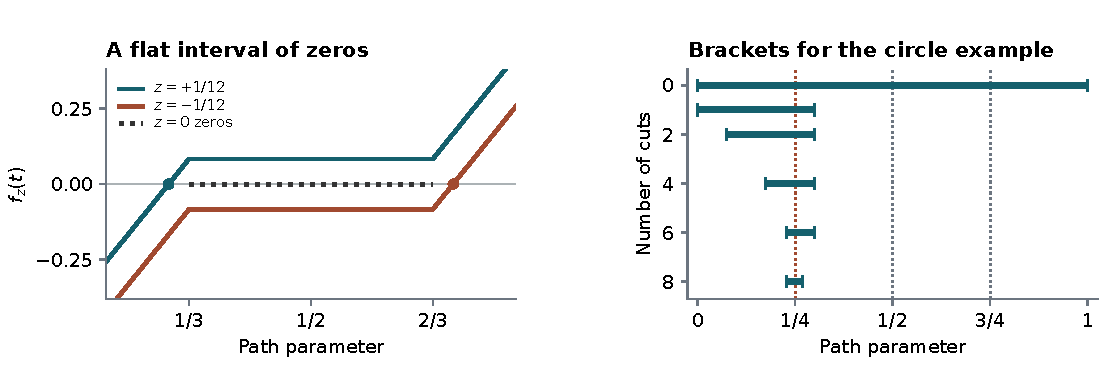
\includegraphics[width=0.97\linewidth]{figures/root_selection.pdf}
\caption{On the left the parameter \(z\) moves a flat segment through zero. The unique roots of the positive and negative perturbations approach different ends of the segment. On the right each horizontal line is the bracket actually retained by the polynomial probe for the unit-circle example. The vertical lines mark the three exact crossing times.}\label{fig:crossings}
\end{figure}

\paragraph{Arithmetic and Lean implementation.}
A bracket stores two rational times and two integer clearance exponents.
After fixing the presentation, acceptance, bit, center-quarter tests and
the cut are PR. The loop invariant is the conjunction of rational ordering,
two accepted marks, opposite bits, nestedness relative to a frozen starting
bracket, and rational width bounds. Each is a Boolean test after coding.
The analytic soundness of the acceptance test is used on demand outside
this induction. For the difference triangle, rational evaluations, maxima
and the entire triangular table have PR codes. Fix its input table and
degree before induction on the row. The invariant is a bounded conjunction
of the row-entry enclosures, encoded by a single PR bit. Similarly polynomial
difference identities follow by coefficient comparison with finite sums for
the binomial expansion. Fixing the modulus query before each width or
triangle induction suffices for quantifier-free induction.

The module \texttt{TopologyCase.lean} proves the bracket step, iteration
invariant, three-step estimate, rate $2^n w_{3n}\le w_0$, and both ingredients of (*) in Lean over rational numbers.
Its \texttt{horner\_top\_difference} proves the exact $d$th difference
identity for every coefficient list and arithmetic progression, and
\texttt{polynomial\_probe\_bound} combines that identity with the signed
enclosure of the difference triangle.

There is also an object derivation for the polynomial identity itself.
In \texttt{TopologyObject.lean}, \texttt{CrossingObject.top\_difference}
constructs a \texttt{Prf PRAAx} of the signed integer equation for every
externally fixed degree and arbitrary integer terms for the coefficients,
origin and step. It interprets the difference fold and Horner evaluation in
the ring of differences of the iPRA term model, proves the identity there,
and applies the repository's \texttt{ZT.derive}. For rational inputs take
a positive common denominator $B_0$, write $x=X/B_0$, $h=H_0/B_0$ and the
coefficients as $b_j/B_0$. Multiplying by $B_0^{d+1}$ turns the sampled
polynomial into $\sum_{j=0}^d b_j B_0^{d-j}(X+iH_0)^j$ at sample $i$.
This directly specifies the signed integer instance to use. Transport back
amounts to cancellation of the positive denominator. The object file
produces the signed polynomial equation. Rational clearing and the
enclosure inequality still need object proofs.

To complete the bracket derivations,
instantiate rational comparisons by cross multiplication on positive
denominators, lift addition and multiplication of signed pairs, and
use these identities for each branch of \texttt{cut\_spec}. Apply
quantifier-free induction to the compiled good-state bit to obtain the
iteration lemma and twice to the width and difference folds. The remaining
analytic interfaces for a general Jordan input are the bit's
positive-clearance stability, the forward and inverse moduli, and the
evaluator error estimates. The packet supplies human arguments for the
Jordan interface. The object derivations still to be constructed cover this
Jordan interface, the rational inequalities and the specialized bracket
inductions.

\section{Residues at primitive-recursively named singularities}
\label{sec:namedresidue}

The residue theorem in the repository takes its singularity centres in
$\mathbb Q(i)$. Its extension to rectifiable curves retains that restriction.
A pole of a rational function with rational coefficients, for example
$+\sqrt{2}$ for $1/(z^2-2)$, need not have rational coordinates.
There are two different uses of the centre in the proof. Laurent
coefficients use it as an origin, while the planar filling algorithm
compares coordinates to draw a mesh. We translate the analytic origin
by a name and draw the mesh around one rational sample. A strip joining
the two contours proves that the computed residue is the coefficient at
the intended origin.

\paragraph{The rational case used below.}
Write $Q_t(c)=\{z:\lVert z-c\rVert_\infty\le t\}$ and put
$|z|_1=|\Re z|+|\Im z|$. Norms in error estimates below are $|\cdot|_1$.
Two results from the repository's
\href{https://github.com/VladimirReshetnikov/ProveIt/blob/5f3be02388442f16487d2dc5c2529961dd783d2b/Logic/PrimitiveRecursiveArithmetic/docs/proofs/analysis/cauchy_residue_ipra/report.tex}{Cauchy and residue report}
are used as mathematical lemmas. First, the integral on the boundary of
a finite rational triangle chain is zero under a uniform first-order
remainder estimate on its carrier. Second, on the rational annulus
$Q_{8r}(0)\setminus\operatorname{int} Q_{r/8}(0)$, the same effective
holomorphy data give Laurent coefficients $a_m$, a unique expansion on
$\partial Q_r(0)$, and $\int_{\partial Q_r(0)}g=2\pi i a_{-1}$.
The annular result derives the coefficients by expanding the two separated
Cauchy kernels on the outer and inner boundary. Both finite geometric
remainders have ratio at most $1/2$. For inner and outer magnitude bounds
at most $M$, the $2N$ terms with indices $-N,\ldots,N-1$ have uniform
error at most $40M2^{-N}$. The moment integral of each integer power
vanishes except for $z^{-1}$, whose integral is $2\pi i$. The linked
report gives the human proofs in its sections on the annular Cauchy
formula and the final residue error budget.

\subsection{Translating a holomorphic chart}

A name $A(n)\in\mathbb Q(i)$ for $a$ is a fixed PR function satisfying
$|A(m)-A(n)|_1\le 2^{-m}+2^{-n}$. A holomorphic chart on a rational
carrier supplies PR evaluators $F(z,n),D(z,n)$, each coherent with
error $2^{-n}$, magnitude bounds $M,B$, and nondecreasing PR moduli
$\nu,\mu$. In name notation the conditions at rational points $z,w$ are
\begin{align*}
 |w-z|_1\le 2^{-\nu(k)}
   &\ \Longrightarrow\ |f(w)-f(z)|_1\le 2^{-k},\\
 |w-z|_1\le 2^{-\mu(k)}
   &\ \Longrightarrow\ |f(w)-f(z)-f'(z)(w-z)|_1
                      \le 2^{-k}|w-z|_1 .
\end{align*}
The first bound at sample precisions $n,m$ has extra slack $2^{-n}+2^{-m}$.
The second at a common precision $n$ has extra slack
$2^{-n}(2+|w-z|_1)$. These clauses, with the two coherence and magnitude
bounds, are first-order statements on rational codes.

\paragraph{Lemma (a modulus for the derivative).}
On that carrier $\mu_D(k)=\mu(k+2)$ works for $f'$. Indeed, let
$h=w-z\ne0$, $d=|h|_1$. Add the two first-order remainders, one in
each direction, and obtain
$|(f'(z)-f'(w))h|_1\le 2\cdot 2^{-(k+2)}d$ when
$d\le 2^{-\mu(k+2)}$. For $h=x+iy$ one has
$|h^{-1}|_1=d/(x^2+y^2)\le 2/d$. Submultiplicativity gives the
claimed $2^{-k}$ bound. The zero-displacement case uses coherence at a
single rational point. Division in this argument is a decidable
operation on nonzero rational $h$. At precision $m$ the two remainders
contribute an additional $4(2+d)2^{-m}/d$ after division. This factor
can be budgeted for each rational pair before taking the arbitrary-error
consequence. For example, to make the extra term at most $2^{-v}$, take
$m=v+\sigma(4(2+d)/d)$, where throughout this section
$\sigma(u)$ is the least $s\ge0$ with $2^s\ge\max(1,u)$.
For a nonnegative fraction $p/q$, $q\ge1$, the search is bounded by $p+1$.

\paragraph{Lemma (translation).}
Choose $r>0$ rational, $b$ with $2^{-b}\le r/64$, and
$c=A(b)$. Assume the chart clauses on the rational closed shell
\[
 S(c,r)=\{z:r/16\le\lVert z-c\rVert_\infty\le 9r\}.
\]
For rational $x$ with $r/8\le\lVert x\rVert_\infty\le8r$, the
translated function $g(x)=f(a+x)$ has PR holomorphy data on this
fixed rational annulus. In particular the preceding rational Laurent
theorem applies to $g$.

To construct the data, observe that for every $t\ge b$,
$\lVert A(t)-c\rVert_\infty\le r/32$. Thus $x+A(t)$ belongs to $S(c,r)$
because $r/8-r/32\ge r/16$ and $8r+r/32\le9r$. To produce the value
and derivative samples at precision $n$, use
\[
 t(n)=\max\{b,1+\nu(n+2),1+\mu(n+4)\}
\]
and evaluate $F(x+A(t(n)),n+2)$ and $D(x+A(t(n)),n+2)$.
Every later centre sample is within $2^{1-t(n)}$ of $A(t(n))$.
The input modulus and the derivative lemma make the centre error at
most $2^{-(n+2)}$ in either value. The evaluator contributes at most
another $2^{-(n+2)}$. In fully rational form, compare two output
samples by inserting a common later centre and a common fine evaluator
precision, then discard the arbitrarily small positive slack by
cross-multiplication. Thus the displayed programs each have error
at most $2^{-n}$ and the required coherence. A translated modulus or
first-order bound for $x,y$ follows by evaluating both at the \emph{same}
later centre $A(T)$. Their displacement is exactly $y-x$. Taking
arbitrary rational precision recovers $\nu,\mu$ unchanged. Replacing
the three resulting names by their output samples introduces precisely
the allowed evaluator slack. Magnitude bounds transport in the same
way. If two input names represent the same centre, the common-sample
comparison with $\nu$ and $\mu_D$ gives equal translated names wherever
the indicated shells are certified.

\subsection{The moving-centre residue theorem}

Let $\Gamma$ be a closed rational polygonal chain and let $A_j(n)$
name finitely many centres $a_j$ (jointly PR in $j,n$ if their number is
a parameter). For each $j$ choose $r_j,b_j,c_j$ as above.
Assume that the $Q_{9r_j}(c_j)$ are pairwise disjoint and miss $\Gamma$.
Give integer weights $w_j$ and a rational triangle chain $T$ satisfying
the finite oriented-boundary identity
\[
 \partial T=\Gamma-\sum_j w_j\partial Q_{r_j}(c_j).
\]
Subdivisions at common rational vertices are allowed. Require
$\lVert z-c_j\rVert_\infty\ge r_j/16$ throughout the carrier of $T$,
and give the holomorphic chart data for $f$ on that carrier and
the shells $S(c_j,r_j)$, with compatible values on overlaps.
Distances and domains here refer to rational cells. Such a filling for
a rectangle with square holes can be produced by drawing the horizontal
and vertical side lines and splitting each retained rectangle into
two triangles. Holomorphy on the carrier of the filling is essential.

\paragraph{Theorem.}
For each $j$, the translated local chart constructs the Laurent
coefficient $R_j$ of degree $-1$ at $a_j$. With name equality
interpreted at every requested precision,
\[
 \int_\Gamma f(z)\,dz=2\pi i\sum_j w_j R_j,\qquad
 w_j=(2\pi i)^{-1}\int_\Gamma \frac{dz}{z-a_j}.
\]
Here $R_j$ is the coefficient of the presented annulus centred at $a_j$.
When the data extend to a punctured neighbourhood of $a_j$ as specified
below, it is the residue of that point. This includes isolated essential
singularities.

\paragraph{Proof.}
Fix $j$ and suppress its index. For $n\ge b$, join the four vertices
of $Q_r(c)$ to the corresponding translated vertices of $Q_r(A(n))$.
Each of the four quadrilaterals is a signed pair of rational triangles.
Its points are of the form $c+x+t(A(n)-c)$ with $x$ on the corresponding
edge of $Q_r(0)$ and $0\le t\le1$. Their distances from $c$ lie between
$r-r/32$ and $r+r/32$ in the sup norm. Thus Cauchy's triangle theorem
applies there, including to degenerate panels. The interior diagonals
and the four connector edges cancel with opposite signs, giving the
exact equality of the integrals on the two rational squares.

The difference between the integral over $\partial Q_r(A(n))$ and
$\int_{\partial Q_r(0)}g(x)\,dx$ has norm at most $8r2^{-u}$ whenever
$n\ge\max(b,1+\nu(u))$. Indeed its two integrands in the fixed $x$
coordinate are within $2^{-u}$ at every rational quadrature node by
the common-later-centre argument. The increments in each finite edge
sum coincide and their total norm is $8r$. The quadrature error on
either side has its supplied modulus and can be made arbitrarily small.
This proves equality for the translated square. By the translation lemma
and the rational annular theorem, its integral is $2\pi iR_j$.
Applying Cauchy to $T$ and using the boundary identity now gives the
first formula.

For the second formula apply the same chain calculation to
$k_j(z)=(z-a_j)^{-1}$. On $T$ and its own shell the distance to $a_j$
is at least $r_j/16-r_j/32$. The disjoint outer squares keep
$k_j$ holomorphic throughout every other local square. The inverse
evaluator is effective here. When the sup distance has lower bound
$\delta>0$, take centre error at most $\delta/2$, use
$|v^{-1}|_1\le2/\lVert v\rVert_\infty$ and the inverse difference
identity to budget its value error. Squaring gives derivative
$-v^{-2}$. The identity
$(v+h)^{-1}-v^{-1}+h/v^2=h^2/(v^2(v+h))$
gives a remainder constant $U^3$ for any common endpoint inverse bound
$U$. In the translated chart at $a_j$ this kernel is $1/x$ and has
residue one. Its integral around each other square vanishes by its
two-triangle filling. The second formula follows. In particular changing
a rational filling or its subdivision gives the same integers since
these normalized integral names depend only on $a_j$ and $\Gamma$.
Independence of radius follows by Cauchy on the intervening annulus
in translated coordinates.\hfill$\square$

\paragraph{From an annular coefficient to a point residue.}
A single shell can surround several singularities. For example,
$(z-d)^{-1}$ with $0<|d-a|_1<r/64$ contributes one to the
annular coefficient around $a$, although the function is regular at $a$.
A sufficient punctured-germ presentation consists of the preceding shell
data for every $r_m=2^{-m}r$, using $b_m=b+m$ and $c_m=A(b_m)$,
jointly PR in $m$ and agreeing on overlaps. In translated coordinates
the adjacent evaluations agree on the common annulus by the
common-later-centre calculation. The square annulus between
half-sides $r_m/2$ and $r_m$ lies in that common annulus, so Cauchy's
theorem on its rectangular filling identifies successive coefficient
integrals. The common value is the coefficient at the isolated point.
For a numerical depth $m$ and precision $q$, sum the $m$ adjacent
differences at precision $q+1+\sigma(m+1)$. This proves independence of
depth with a rational prefix invariant. The positive gap around each
other centre is retained at all the smaller scales.

\paragraph{Rectifiable curves.}
The same result holds for a closed PR-named curve $\gamma$ with
a PR continuity modulus $\nu_\gamma$ and a supplied upper bound on the
sum of its increments' norms over every dyadic partition. Give a
positive rational $\rho$ such that $f$ has the chart data on the
$\rho$-collar of the curve and
$\lVert\gamma(t)-a_j\rVert_\infty\ge\rho$ for every $j,t$.
Choose $2^{-C}\le\rho/8$, $m=\nu_\gamma(C)$, and join
$2^{-C}$-accurate rational samples at the times $i/2^m$ to obtain a
rational polygon $P$, using the same sample at both endpoints. On each
subinterval both endpoint samples are within $2\cdot2^{-C}$ of
$\gamma(t)$, so $|P(t)-\gamma(t)|_1\le\rho/4$ by convexity.
The linear homotopy from $\gamma$ to $P$ has its $\rho/2$-collar
in the chart and at sup distance at least $\rho/4$ from all centres.
For a PR modulus use $\max(\nu_\gamma(k+2),k+2+d)$ where $2^d$ bounds
one, $\rho/4$, and the greatest speed on the polygon's parameter
segments. Changing $t$ and then the homotopy parameter in its affine
formula proves this bound. The rational-grid homotopy theorem in the
linked report identifies the two contour integrals, for $f$ and for
each inverse kernel individually. Whenever $P$ has the filling and
shell certificates above, the same coefficients and integers therefore
give the value and the windings for $\gamma$.

\paragraph{Precision and induction.}
For a target $2^{-q}$ take
$u=q+4+\sigma(1+\sum_j8r_j|w_j|)$. The total weighted error of replacing
moving contours by frozen samples is then at most $2^{-q-4}$.
A local Laurent truncation of order
$N\ge1+q+4+\sigma(1+\sum_j 8r_j|w_j|40M_j)$ gives the same
bound on the accumulated truncation error. For the residual of Cauchy's theorem on $T$ and on all rational
translation panels, give each constituent triangle error at most
$2^{-q-4-\sigma(1+L)}$ in the upstream triangle schedule, where $L$
is the sum of absolute triangle multiplicities in $T$ plus
$8\sum_j|w_j|$ for the panels. This bounds their combined residual by
$2^{-q-4}$. Finally set $W=\sum_j|w_j|$ and
$B_*=\sum_j |w_j|8r_jM_j$. The local coefficient integral and
$|(2\pi i)^{-1}|_1\le1$ give $\sum_j|w_j|\,|R_j|_1\le B_*$.
If the sampled $\pi$ has magnitude at most five, and its error and the
errors in the outer integral and individual residues are
$\eta_\pi,\eta_\Gamma,\eta_R$, the additional error in the equality is
at most $\eta_\Gamma+2B_*\eta_\pi+10W\eta_R$. Use $q+4$ bits for the
outer integral, $q+4+\sigma(1+2B_*)$ for $\pi$, and
$q+4+\sigma(1+10W)$ for the residue names, with the rational-case
schedules for quadrature and numerical coefficient evaluation. Even
adding all six indicated error allowances gives less than $2^{-q}$.
The proof of cancellation fixes an elementary oriented edge and inducts
on a partial sum of signed incidences. The sum estimate inducts on the
rational accumulator of the norm bounds at fixed precision. The
analytic hypotheses are used by instantiation at the rational sample
points. Equality of names means agreement to all rational accuracies.
A violated rational inequality has a decidable positive gap and a PR
precision that detects it.

\paragraph{Example.}
Take $a=\sqrt2$, $f(z)=(z^2-2)^{-1}$, and let $\Gamma$ be the positive
boundary of $[1,2]\times[-1/2,1/2]$. Use the lower dyadic name
$A(n)=2^{-n}\lfloor\sqrt{2\cdot 4^n}\rfloor$, obtained by bounded
integer search, and put $r=1/64$, $b=12$, $c=181/128$.
The outer square of half-side $9r$ lies strictly inside the rectangle.
The four lines supporting the hole divide the rectangle into nine cells.
Deleting the middle cell gives a filling of sixteen triangles with
weight one. On the carrier and shell the factor $z-a$ is bounded away
from zero by the clearance above and $\lVert z+a\rVert_\infty\ge1$
by its real part. The partial-fraction identity
\[
 \frac1{z^2-2}=\frac1{2a}\left(\frac1{z-a}-\frac1{z+a}\right)
\]
supplies effective data by the inverse estimate, and gives
$R=1/(2a)$ because the second summand is holomorphic across the
whole square. Thus $\int_\Gamma dz/(z^2-2)=\pi i/\sqrt2$.
The arithmetic fact $a^2=2$ follows directly from
$A(n)^2\le2<(A(n)+2^{-n})^2$ and $A(n)\le2$.

\paragraph{Lean implementation path.}
The host file \texttt{ComplexCase.lean} defines an incidence functional
on ordered vertex pairs, the boundary of one oriented triangle, and
the signed two-triangle panel. Its lemmas \texttt{strip\_boundary}
and \texttt{closed\_strip} give cancellation for every finite strip,
and \texttt{annulus\_clearance} proves the integer-scaled shell
inequality. The file also proves both taxicab bounds for Gaussian integer
multiplication. Its \texttt{derivative\_variation} lemma recovers the
factor four in the derivative modulus after clearing positive denominators. If $|Ch|_1\le 2E|h|_1$ and $|h|_1>0$, then $|C|_1\le4E$. The companion \texttt{ComplexObject.lean} proves the strip identity in
the repository's object calculus. For an arbitrary externally fixed
path and an incidence table $E$ whose entries are signed pairs of open
terms, \texttt{ResidueObject.closed\_strip} constructs a
$\Gamma\vdash_{\mathsf{PRAAx}}$ derivation of the signed boundary
equation. Its \texttt{square\_strip} specialization gives the eight
triangles used above. The proof interprets the incidence expressions
in the repository's ring of formal differences, cancels them there, and
applies \texttt{ZT.derive}. An implementation of the geometry must still
supply the incidence terms for the chosen rational test edge, with
normalization of endpoints and signed comparisons. A single uniform
object formula for coded paths of variable length would additionally
use a quantifier-free prefix induction. Next implement
$|\cdot|_1,\lVert\cdot\rVert_\infty$,
the rational inverse and the two displayed scheduling functions by
cross-multiplication and bounded recursion. The derivative lemma uses
the two instantiated remainder inequalities and the inequality
$(|x|+|y|)^2\le2(x^2+y^2)$.
The translated samples are the displayed compositions of PR functions.
With these arithmetic lemmas the remaining subgoals are the
rational triangle and Laurent derivations from the upstream roadmap,
followed by universal elimination at the translated programs and
the finite weighted sum. The included Python example checks the grid
boundary, all triangle-strip incidences, dyadic brackets, and the
rational-proxy partial-fraction identity exactly.

\section{Verification and remaining proof obligations}\label{sec:verification}

A Lean proof concerning numbers or functions in its standard library is a proof about the algorithm in the metatheory. A term of type \(\Gamma\vdash_{\mathsf{PRAAx}}\phi\) additionally constructs a proof in the specific arithmetic of the repository. Table~\ref{tab:verify} records this distinction. In both settings the compilation target is Lean 4.32.0. Exact rational examples exercise the constructions separately.

\begin{table}[ht]
\centering\small
\renewcommand{\arraystretch}{1.15}
\begin{tabular}{@{}p{0.20\linewidth}p{0.37\linewidth}p{0.36\linewidth}@{}}
\toprule
Application & Object calculus & Standard Lean \\
\midrule
Metric kernels & Minimum transfer over two variable numerical horizons. Finite disjunctive cover and exact diagonal calculation for an unrolled row. & The finite comparison theorem for a nonexpansive formula is in the model module.\\
Continuous logic & Transport of upper cuts through arbitrary fixed finite nests of lattice connectives and quantifiers, given the atomic implication proofs. & Two-sided numerical transfer for arity-indexed formulas, and construction of a minimizing list entry.\\
Jordan crossing & Polynomial forward-difference identity with integer term coefficients and a specified degree. & Bracket iteration, width rate, exact Horner difference identity, and sample-size lower bound.\\
Residues & Signed incidence cancellation on a rational contour strip after specifying the finite edge data. & Strip telescoping, shell clearance, Gaussian norm inequalities and derivative-variation estimate.\\
\bottomrule
\end{tabular}
\caption{Scope of the supplied formal lemmas. The object results allow numerical parameters in the terms.}\label{tab:verify}
\end{table}

\paragraph{How to read the object endpoints.}
For \texttt{MetricKernel.Row.cover\_transfer}, fix two nonempty row shapes \(s,r\) externally. Their entries and error \(e\) are arbitrary numerical terms. On a common scale the actual formula is
\[
 \bigwedge_{x\in r}\ \bigvee_{y\in s}\; y\le x+e
 \quad\longrightarrow\quad \min s\le\min r+e.
\]
The term for the binary minimum is \(a\mathbin{\dot-}(a\mathbin{\dot-}b)\), where \(\dot-\) denotes truncated subtraction. The proof internally splits on the derived order-totality disjunction. It never asks the metatheory to pick which entry wins. The companion \texttt{diagonal\_exact} takes lower-bound proofs for all alternatives and an equality proof for the specified diagonal. For a probe this lower bound is the triangle law of the kernel, and the diagonal equality uses \(d(a,a)=0\). The statement handles any externally fixed row shape. For the scalar gluing test, clearing positive denominators and using signed-pair arithmetic implements the two comparisons in \eqref{eq:glue} and its witness. The global kernel laws, the converse representation theorem and the interval formula have human proofs in this report.

\paragraph{A kernel-checked theorem with both horizons internal.}
The main reusable arithmetic endpoint is \texttt{UniformMinimum.transfer\_closed}. Fix arbitrary binary PR symbols \(f,g\) and put \(M_f(K,x)=\min_{i\le K} f(i,x)\). The checked conclusion is an empty-context proof in \(\mathsf{PRAAx}\) of the universal closure in \(K,H,x,y,e\) of
\[
 \big[\forall j\le H\ \exists i\le K\quad f(i,x)\le g(j,y)+e\big]
 \quad\Longrightarrow\quad M_f(K,x)\le M_g(H,y)+e .
\]
The companion \texttt{symmetric\_closed} proves both inequalities from the two directed covers. Both scans are actual PR terms, starting at index zero. To see why a bounded existential in the premise is harmless, first fix a source index \(i\). Induct on \(k\) with quantifier-free invariant \(i\le k\Rightarrow M_f(k,x)\le f(i,x)\). The new index either equals \(i\) or retains the previous bound. For each \(j\le H\) eliminate its covering witness locally. This yields \(M_f(K,x)\le g(j,y)+e\). Put \(z=M_f(K,x)\) and induct once more with invariant \(j\le H\Rightarrow z\le M_g(j,y)+e\). At a successor the minimum is one of its two arguments, both already bounded below after adding \(e\). Universal closure comes after these inductions. In particular, the proof produces the numerical inequality without a choice function for the matches.

\paragraph{From a presentation to a closed sentence.}
Fix the PR codes for the metric, nets, atomic evaluators, moduli and any other program supplied by the chosen case. Encode the finite tables of rational outputs together with one positive denominator (the product of the entry denominators suffices). Each cost in a comparison then has one integer representative. Translate signed values by a common nonnegative offset if a natural minimum is used; both sides of the min-transfer inequality acquire the same offset. Rationals with independent denominators also have a repository-native \texttt{RationalArgmin} implementation. Store a quantified assignment or bracket state in the repository's pairing/sequence coding and apply bounded reflection to the PR test for its validity. For variable-size finite comparisons, use a minimum over \(0,\ldots,M\), where \(M\) is the last valid index, with a separate guard for a possibly empty incoming list.

The next arithmetic statements are the displayed cross-stage estimates, with only the actual finite bound or term for each requested index used in a proof. For example, instantiate the one-way minimum inequality on the two nets with scores \(K_i(x,b)+H_i(b,z)\), the computed common denominator and error \(2\max(h_i,h_j)+2(h_i+h_j)\). Produce the required index using the stated net cover and prove its score bound by two uses of \eqref{eq:cost-law}. Repeat with the levels reversed and apply the two-step shift. Generalizing \(i,j,x,z\) yields an actual object target for regularity of composition. For model formulas perform the same pair of instantiations at a binder using the child theorem in place of the cost estimate. This is a structural proof generator on fixed formulas. The rows, covers, scores and bounds remain numerical data in its uniform version. For topology and residues the implementation paragraphs of the respective sections identify the additional arithmetic and geometric lemmas. Each output sentence can retain its presentation contracts as antecedents. Obtaining a closed theorem for one specific presentation additionally requires object proofs of those contracts.

The repository's \href{https://github.com/VladimirReshetnikov/ProveIt/blob/5f3be02388442f16487d2dc5c2529961dd783d2b/Logic/PrimitiveRecursiveArithmetic/Derivations/README.md}{arithmetic derivation library} and \href{https://github.com/VladimirReshetnikov/ProveIt/blob/5f3be02388442f16487d2dc5c2529961dd783d2b/Logic/PrimitiveRecursiveArithmetic/ConciseIPRA/README.md}{presentation and transfer theorems} identify the ordinary proof predicate and its connection to the scalar core. Proofs of the general Jordan separation interface and of rational triangle Cauchy and Laurent evaluation remain analytic obligations for a complete deep embedding. Our use of these results in the corresponding human proofs is relative to the hypotheses stated in those sections. Independent concrete examples, including the scalar sign proof and the circle, avoid the full Jordan interface.

\paragraph{Further research questions.}
Can the probe estimate in Theorem~\ref{thm:probe} be made adaptive by refining only cells whose observed discrepancy is near the current maximum, with a PR bound derived from local moduli? Which effective quasianalytic or sublevel-set estimates can replace the polynomial forward-difference bound and still give a middle-bracket probe? For known separated zero clusters of a holomorphic function, can a cluster boundary yield a PR residue sum without any individual centre names? These questions concern different missing data: a stopping bound for refinement, a supply of clear points, and a local analytic chart for a whole cluster.

\end{document}
